\documentclass[aspectratio=169,11pt]{beamer}

% Theme and colors
\usetheme{Madrid}
\usecolortheme{whale}
\setbeamertemplate{navigation symbols}{}
\setbeamertemplate{footline}[frame number]

% Packages
\usepackage[utf8]{inputenc}
\usepackage[T1]{fontenc}
\usepackage{graphicx}
\usepackage{booktabs}
\usepackage{amsmath}
\usepackage{hyperref}
\usepackage{tikz}
\usetikzlibrary{shapes,arrows,positioning,calc,fit,backgrounds,decorations.pathmorphing,patterns}
\usepackage{siunitx}
\usepackage{xcolor}
\usepackage{array}

% Custom colors
\definecolor{questionbg}{RGB}{255,248,220}
\definecolor{questionborder}{RGB}{255,193,7}

% Title information
\title[EECE5155 -- Module 7]{Data Storage for IoT}
\subtitle{Module 7: From Raw Bytes to Queryable Knowledge}
\author{Eduardo Baena}
\date{Spring 2026}
\institute{Northeastern University\\Department of Electrical and Computer Engineering\\
\texttt{e.baena@northeastern.edu}}

\begin{document}

% Title slide
\begin{frame}
    \titlepage
    \vspace{-1cm}
    \begin{center}
        \textbf{EECE5155: Wireless Sensor Networks and the Internet of Things}
    \end{center}
\end{frame}

%==============================================================================
\section{Learning Objectives}
%==============================================================================

\begin{frame}{Learning Objectives}
    \textbf{By the end of this module, you should be able to:}

    \vspace{0.2cm}
    \begin{enumerate}
        \item \textbf{Classify} IoT data storage patterns: hot path, warm path, cold path
        \item \textbf{Compare} storage technologies: time-series DBs, relational, NoSQL, object storage, data lakes
        \item \textbf{Justify} the choice of InfluxDB, TimescaleDB, or Apache Parquet for a given scenario
        \item \textbf{Design} a Lambda/Kappa architecture for IoT data pipelines
        \item \textbf{Evaluate} edge-to-cloud storage hierarchies and data lifecycle strategies
        \item \textbf{Apply} data compression and retention policies to constrained IoT deployments
    \end{enumerate}

    \vspace{0.1cm}
    \begin{alertblock}{Context}
        Data flows from device to broker (Mod.\ 6). Now: where does it land? How is it stored, indexed, and made queryable at scale?
    \end{alertblock}
\end{frame}

%==============================================================================
\section{Outline}
%==============================================================================

\begin{frame}{Outline}
    \tableofcontents
\end{frame}

%==============================================================================
\section{The IoT Data Storage Problem}
%==============================================================================

\begin{frame}{The IoT Data Storage Problem}
    \small
    \textbf{IoT data is unlike any data your SQL class prepared you for:}

    \vspace{0.05cm}
    \begin{columns}
        \column{0.5\textwidth}
        \textbf{Volume:}
        \begin{itemize}\setlength{\itemsep}{0pt}
            \item 10k sensors at 1~Hz = \textbf{864M readings/day}
            \item Smart city, 100k nodes = \textbf{8.6B/day}
            \item IIoT generates \textbf{petabytes/year}
        \end{itemize}

        \vspace{0.05cm}
        \textbf{Velocity:}
        \begin{itemize}\setlength{\itemsep}{0pt}
            \item High-freq: vibration sensors at 10~kHz
            \item Low-freq: soil moisture every 30~min
            \item \textbf{Bursty}: 10k devices reconnect after outage
        \end{itemize}

        \column{0.5\textwidth}
        \textbf{Variety:}
        \begin{itemize}\setlength{\itemsep}{0pt}
            \item Structured: temperature, pressure
            \item Semi-structured: JSON payloads
            \item Unstructured: images, audio
            \item Sparse: battery devices sleep
        \end{itemize}

        \vspace{0.05cm}
        \textbf{Veracity:}
        \begin{itemize}\setlength{\itemsep}{0pt}
            \item Sensor noise, stuck values
            \item Late arrivals (out-of-order timestamps)
            \item Duplicate messages (QoS~1)
            \item Missing data (network outages)
        \end{itemize}
    \end{columns}

    \begin{alertblock}{The 4 Vs}
        Volume + Velocity + Variety + Veracity. No single database handles all four optimally.
    \end{alertblock}
\end{frame}

%==============================================================================
\section{Hot, Warm, and Cold Paths}
%==============================================================================

\begin{frame}{Hot Path / Warm Path / Cold Path}
    \textbf{The fundamental architecture pattern for IoT data:}

    \vspace{0.2cm}
    \begin{center}
    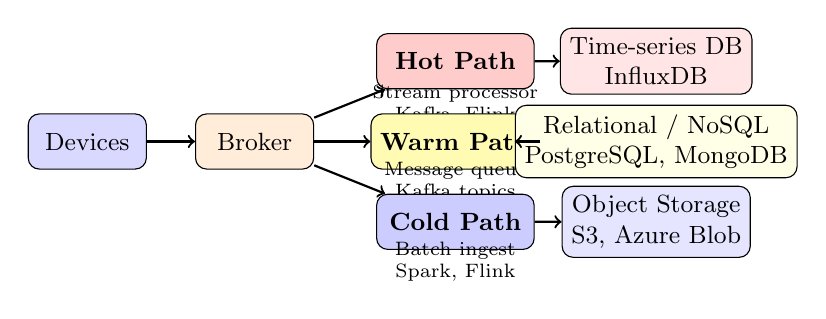
\begin{tikzpicture}[scale=0.85, every node/.style={font=\small}]
        % Device
        \node[draw, fill=blue!15, minimum width=1.5cm, minimum height=0.7cm, rounded corners] (dev) at (0,0) {Devices};
        % Broker
        \node[draw, fill=orange!15, minimum width=1.5cm, minimum height=0.7cm, rounded corners] (broker) at (2.5,0) {Broker};
        % Arrow
        \draw[->, thick] (dev) -- (broker);

        % Hot path
        \node[draw, fill=red!20, minimum width=2cm, minimum height=0.7cm, rounded corners] (hot) at (5.5,1.2) {\textbf{Hot Path}};
        \node[font=\scriptsize, align=center] at (5.5,0.55) {Stream processor\\Kafka, Flink};
        \node[draw, fill=red!10, minimum width=2.2cm, minimum height=0.6cm, rounded corners, align=center] (hotdb) at (8.5,1.2) {Time-series DB\\InfluxDB};
        \draw[->, thick] (broker) -- (hot);
        \draw[->, thick] (hot) -- (hotdb);

        % Warm path
        \node[draw, fill=yellow!30, minimum width=2cm, minimum height=0.7cm, rounded corners] (warm) at (5.5,0) {\textbf{Warm Path}};
        \node[font=\scriptsize, align=center] at (5.5,-0.6) {Message queue\\Kafka topics};
        \node[draw, fill=yellow!10, minimum width=2.2cm, minimum height=0.6cm, rounded corners, align=center] (warmdb) at (8.5,0) {Relational / NoSQL\\PostgreSQL, MongoDB};
        \draw[->, thick] (broker) -- (warm);
        \draw[->, thick] (warm) -- (warmdb);

        % Cold path
        \node[draw, fill=blue!20, minimum width=2cm, minimum height=0.7cm, rounded corners] (cold) at (5.5,-1.2) {\textbf{Cold Path}};
        \node[font=\scriptsize, align=center] at (5.5,-1.8) {Batch ingest\\Spark, Flink};
        \node[draw, fill=blue!10, minimum width=2.2cm, minimum height=0.6cm, rounded corners, align=center] (colddb) at (8.5,-1.2) {Object Storage\\S3, Azure Blob};
        \draw[->, thick] (broker) -- (cold);
        \draw[->, thick] (cold) -- (colddb);
    \end{tikzpicture}
    \end{center}

    \begin{alertblock}{Key Insight}
        Hot path = milliseconds latency, short retention. Cold path = hours latency, years retention. Most production systems need all three.
    \end{alertblock}
\end{frame}

\begin{frame}{Hot / Warm / Cold Path: Characteristics}
    \vspace{0.1cm}
    \begin{center}
    \footnotesize
    \begin{tabular}{p{2cm}p{3cm}p{3cm}p{3.5cm}}
        \toprule
        & \textbf{Hot Path} & \textbf{Warm Path} & \textbf{Cold Path} \\
        \midrule
        \textbf{Latency} & $<$100 ms & Seconds--minutes & Hours--days \\
        \textbf{Retention} & Hours--days & Days--months & Years \\
        \textbf{Use case} & Alerts, dashboards & Recent queries & ML training, audit \\
        \textbf{Storage} & Time-series DB & SQL / NoSQL & Object storage \\
        \textbf{Cost} & High (fast SSD) & Medium & Low (HDD/tape) \\
        \textbf{Query} & Real-time & Ad-hoc & Batch \\
        \bottomrule
    \end{tabular}
    \normalsize
    \end{center}

    \vspace{0.15cm}
    \begin{columns}
        \column{0.5\textwidth}
        \textbf{Example: Smart Grid}
        \begin{itemize}
            \item Hot: fault detection ($<$50 ms)
            \item Warm: billing queries (last 3 months)
            \item Cold: regulatory compliance (10 years)
        \end{itemize}

        \column{0.5\textwidth}
        \textbf{Example: Connected Vehicle}
        \begin{itemize}
            \item Hot: safety alerts, live telemetry
            \item Warm: trip analytics, diagnostics
            \item Cold: crash investigation, ML training
        \end{itemize}
    \end{columns}
\end{frame}

%==============================================================================
\section{Time-Series Databases}
%==============================================================================

\begin{frame}{Time-Series Databases: Why They Exist}
    \small
    \textbf{Why not just use PostgreSQL for IoT data?}

    \vspace{0.1cm}
    \begin{columns}
        \column{0.5\textwidth}
        \textbf{Problems with general-purpose DBs:}
        \begin{itemize}\setlength{\itemsep}{0pt}
            \item B-tree indexes degrade with time-series inserts
            \item No native compression for sensor patterns
            \item No built-in downsampling / retention
            \item Aggregations slow on billions of rows
            \item Schema changes expensive at scale
        \end{itemize}

        \column{0.5\textwidth}
        \textbf{Time-series DB optimizations:}
        \begin{itemize}\setlength{\itemsep}{0pt}
            \item \textbf{LSM tree} / columnar: fast sequential appends
            \item \textbf{Delta+XOR compression}: 10--100$\times$ ratio
            \item \textbf{Downsampling}: raw$\rightarrow$1~min$\rightarrow$1~hr averages
            \item \textbf{Retention policies}: auto-delete old data
            \item \textbf{Time-aware queries}: \texttt{GROUP BY time(1h)}
        \end{itemize}
    \end{columns}

    \vspace{0.1cm}
    \begin{exampleblock}{Gorilla compression (Meta, 2015)}
        Stores 16 bytes of float+timestamp in $\approx$1.37 bytes on average. Used in InfluxDB, Prometheus, VictoriaMetrics.
    \end{exampleblock}
\end{frame}

\begin{frame}{InfluxDB: The IoT Time-Series Standard}
    \small
    \textbf{InfluxDB} (InfluxData, 2013 -- v3.x rewritten 2024):

    \vspace{0.05cm}
    \begin{columns}
        \column{0.5\textwidth}
        \textbf{Key concepts:}
        \begin{itemize}\setlength{\itemsep}{0pt}
            \item \textbf{Measurement}: table analog (e.g., \texttt{temperature})
            \item \textbf{Tags}: indexed metadata (device ID, location)
            \item \textbf{Fields}: sensor values (float, int, string)
            \item \textbf{Timestamp}: nanosecond precision
            \item \textbf{Bucket}: retention-scoped container
        \end{itemize}

        \vspace{0.05cm}
        \textbf{Query language:}
        \begin{itemize}\setlength{\itemsep}{0pt}
            \item \textbf{InfluxQL}: SQL-like (v1.x)
            \item \textbf{Flux}: functional pipeline (v2.x)
            \item \textbf{SQL}: native in v3.x (Arrow Flight)
        \end{itemize}

        \column{0.5\textwidth}
        \textbf{InfluxDB 3.x (2024):}
        \begin{itemize}\setlength{\itemsep}{0pt}
            \item Rewritten in \textbf{Rust} on Apache Parquet
            \item \textbf{S3-compatible} object storage backend
            \item Unlimited tag cardinality
            \item Native SQL + InfluxQL support
            \item InfluxDB Cloud Serverless
        \end{itemize}

        \vspace{0.05cm}
        \begin{alertblock}{Adoption (2026)}
            Used by Tesla, NASA, Cisco, Siemens. \#1 time-series DB by DB-Engines ranking.
        \end{alertblock}
    \end{columns}
\end{frame}

\begin{frame}{TimescaleDB: Time-Series on PostgreSQL}
    \small
    \textbf{TimescaleDB} (2017): PostgreSQL extension for time-series.

    \vspace{0.05cm}
    \begin{columns}
        \column{0.5\textwidth}
        \textbf{Architecture:}
        \begin{itemize}\setlength{\itemsep}{0pt}
            \item \textbf{Hypertables}: auto-partitioned by time
            \item Standard SQL -- transparent to application
            \item \textbf{Continuous aggregates}: pre-computed rollups
            \item \textbf{Compression}: columnar, 90--95\% ratio
            \item \textbf{Data tiering}: auto-move old data to S3
        \end{itemize}

        \vspace{0.05cm}
        \textbf{Key advantage over InfluxDB:}
        \begin{itemize}\setlength{\itemsep}{0pt}
            \item Full SQL + JOINs with relational tables
            \item Existing PostgreSQL tooling, ORMs, drivers
            \item ACID transactions
        \end{itemize}

        \column{0.5\textwidth}
        \textbf{When to choose:}
        \begin{itemize}\setlength{\itemsep}{0pt}
            \item Time-series \textbf{AND} relational queries needed
            \item JOIN sensor data with asset metadata
            \item Team already knows PostgreSQL
            \item Compliance requires ACID
        \end{itemize}

        \vspace{0.05cm}
        \begin{exampleblock}{Real example}
            \texttt{\scriptsize SELECT avg(temp), asset.location}\\
            \texttt{\scriptsize FROM readings JOIN assets}\\
            \texttt{\scriptsize WHERE time > now() - INTERVAL '1h'}\\
            TimescaleDB handles this. InfluxDB cannot JOIN.
        \end{exampleblock}
    \end{columns}
\end{frame}

\begin{frame}{Other Time-Series Databases (2026)}
    \vspace{0.05cm}
    \begin{center}
    \scriptsize
    \begin{tabular}{p{2.6cm}p{3cm}p{3cm}p{2.8cm}}
        \toprule
        \textbf{Database} & \textbf{Architecture} & \textbf{Best for} & \textbf{Notable users} \\
        \midrule
        \textbf{InfluxDB 3.x} & Rust + Parquet + S3 & Cloud IoT, high cardinality & Tesla, NASA \\
        \textbf{TimescaleDB} & PostgreSQL extension & SQL + time-series hybrid & Retail, finance IoT \\
        \textbf{Prometheus} & Pull-based, in-memory & Infrastructure monitoring & Cloud-native ops \\
        \textbf{VictoriaMetrics} & High-perf InfluxDB alt. & Cost-effective at scale & Adtech, telemetry \\
        \textbf{QuestDB} & SIMD columnar, Java & Ultra-fast ingestion & Trading, IoT edge \\
        \textbf{TDengine} & Purpose-built IoT TSDB & Industrial IoT, IIoT & Smart factories \\
        \bottomrule
    \end{tabular}
    \normalsize
    \end{center}

    \vspace{0.1cm}
    \begin{alertblock}{Selection rule}
        Prometheus = monitoring. InfluxDB = cloud IoT. TimescaleDB = hybrid SQL. QuestDB = max ingestion speed at edge.
    \end{alertblock}
\end{frame}

%==============================================================================
\section{NoSQL and Relational Storage}
%==============================================================================

\begin{frame}{NoSQL Storage for IoT: When and Why}
    \small
    \textbf{Not all IoT data is time-series. Not all queries are time-range.}

    \vspace{0.05cm}
    \begin{columns}
        \column{0.5\textwidth}
        \textbf{Document DBs (MongoDB, Couchbase):}
        \begin{itemize}\setlength{\itemsep}{0pt}
            \item JSON documents --- flexible schema
            \item \textbf{Good for:} device metadata, config, heterogeneous payloads
            \item \textbf{Bad for:} high-freq append-only telemetry
            \item Atlas Device Sync: offline-first IoT
        \end{itemize}

        \vspace{0.05cm}
        \textbf{Key-Value DBs (Redis, DynamoDB):}
        \begin{itemize}\setlength{\itemsep}{0pt}
            \item Nanosecond reads/writes
            \item \textbf{Good for:} device state, last-known-value
            \item Redis TimeSeries: lightweight TSDB at edge
        \end{itemize}

        \column{0.5\textwidth}
        \textbf{Wide-column (Cassandra, ScyllaDB):}
        \begin{itemize}\setlength{\itemsep}{0pt}
            \item Partition by device ID, cluster by time
            \item Massive write throughput (millions/s)
            \item \textbf{Good for:} multi-tenant telemetry at hyperscale
            \item \textbf{Bad for:} complex aggregations
        \end{itemize}

        \vspace{0.05cm}
        \begin{exampleblock}{Pattern: last-known-value}
            Redis: \texttt{device:1234:temp} = 23.5\\
            Updated on each MQTT message. Dashboard reads in $<$1~ms.
        \end{exampleblock}
    \end{columns}
\end{frame}

%==============================================================================
\section{Cloud Object Storage and Data Lakes}
%==============================================================================

\begin{frame}{Object Storage: The Cold Path Foundation}
    \small
    \textbf{S3, Azure Blob, Google Cloud Storage} --- the cold path backbone.

    \vspace{0.05cm}
    \begin{columns}
        \column{0.5\textwidth}
        \textbf{Why object storage?}
        \begin{itemize}\setlength{\itemsep}{0pt}
            \item \textbf{Cost:} \$0.023/GB-month vs \$0.10--0.25 for managed DBs
            \item \textbf{Durability:} 99.999999999\% (11 nines)
            \item \textbf{Scale:} unlimited; exabytes in production
            \item S3-compatible: MinIO, Ceph for on-prem
        \end{itemize}

        \vspace{0.05cm}
        \textbf{File format matters:}
        \begin{itemize}\setlength{\itemsep}{0pt}
            \item \textbf{CSV/JSON}: readable but huge, slow queries
            \item \textbf{Apache Parquet}: columnar, 87\% smaller, DuckDB/Spark native
            \item \textbf{Apache ORC}: Hadoop ecosystem
            \item \textbf{Apache Arrow}: in-memory columnar, zero-copy
        \end{itemize}

        \column{0.5\textwidth}
        \textbf{Partitioning strategy:}
        \begin{itemize}\setlength{\itemsep}{0pt}
            \item \texttt{\scriptsize s3://bucket/year=2026/month=02/}
            \item Partition pruning: query only relevant files
            \item \textbf{Hive-style partitioning} universal
        \end{itemize}

        \vspace{0.05cm}
        \begin{alertblock}{Apache Parquet in 2026}
            Standard for IoT cold storage. InfluxDB~3.x stores natively in Parquet. DuckDB queries S3 Parquet in-place.
        \end{alertblock}
    \end{columns}
\end{frame}

\begin{frame}{Data Lakes and Lakehouses for IoT}
    \small
    \textbf{Data Lake} = raw data in object storage. \textbf{Lakehouse} = lake + ACID + schema.

    \vspace{0.05cm}
    \begin{columns}
        \column{0.5\textwidth}
        \textbf{Data Lake (S3 + raw Parquet):}
        \begin{itemize}\setlength{\itemsep}{0pt}
            \item Cheap, schema-on-read
            \item Risk: becomes a ``data swamp''
            \item No ACID, no upserts, no deletes
            \item Hard to manage schema evolution
        \end{itemize}

        \vspace{0.05cm}
        \textbf{Lakehouse formats (2024--2026):}
        \begin{itemize}\setlength{\itemsep}{0pt}
            \item \textbf{Apache Iceberg}: ACID, time-travel, schema evolution. AWS, Apple, Netflix.
            \item \textbf{Delta Lake}: Databricks-origin, Linux Foundation
            \item \textbf{Apache Hudi}: streaming upserts on S3
        \end{itemize}

        \column{0.5\textwidth}
        \textbf{Why Iceberg for IoT?}
        \begin{itemize}\setlength{\itemsep}{0pt}
            \item Late sensor data: \textbf{upserts} without file rewrite
            \item Firmware bug: \textbf{delete} bad readings
            \item \textbf{Time-travel}: query any historical snapshot
            \item Schema evolution: add metric without migration
        \end{itemize}

        \vspace{0.05cm}
        \begin{exampleblock}{2026 Status}
            AWS Glue + Iceberg = dominant IoT lake pattern. Azure: Delta Lake. Both: Spark, DuckDB, Trino.
        \end{exampleblock}
    \end{columns}
\end{frame}

%==============================================================================
\section{Edge Storage}
%==============================================================================

\begin{frame}{Edge Storage: Why Store Locally?}
    \small
    \textbf{Not everything should go to the cloud immediately.}

    \vspace{0.05cm}
    \begin{columns}
        \column{0.5\textwidth}
        \textbf{Why edge storage?}
        \begin{itemize}\setlength{\itemsep}{0pt}
            \item \textbf{Connectivity:} intermittent networks
            \item \textbf{Latency:} closed-loop control needs $<$10~ms
            \item \textbf{Cost:} cloud egress = \$0.09/GB (AWS)
            \item \textbf{Bandwidth:} 10~kHz vibration = 80~kB/s/channel
            \item \textbf{Privacy:} GDPR, HIPAA local processing
            \item \textbf{Resilience:} operate when offline
        \end{itemize}

        \column{0.5\textwidth}
        \textbf{Edge storage technologies:}
        \begin{itemize}\setlength{\itemsep}{0pt}
            \item \textbf{SQLite}: embedded, ACID. Millions of IoT devices
            \item \textbf{InfluxDB IOx}: lightweight, Raspberry Pi / Jetson
            \item \textbf{Redis TimeSeries}: in-memory at gateway
            \item \textbf{QuestDB}: columnar on edge server
            \item \textbf{RocksDB}: key-value, used in EMQX broker
        \end{itemize}

        \vspace{0.05cm}
        \begin{alertblock}{Design pattern}
            Store locally $\rightarrow$ process $\rightarrow$ upload \textbf{summaries}. Only anomalies go to cloud.
        \end{alertblock}
    \end{columns}
\end{frame}

\begin{frame}{Store-and-Forward and Sync Patterns}
    \small
    \textbf{What happens when the network goes down?}

    \vspace{0.05cm}
    \begin{columns}
        \column{0.5\textwidth}
        \textbf{Store-and-forward:}
        \begin{itemize}\setlength{\itemsep}{0pt}
            \item Buffer data locally during outage
            \item Replay to cloud when connectivity restores
            \item MQTT QoS~1/2 persistent sessions: built-in
            \item Broker buffers limited --- disk persistence needed
        \end{itemize}

        \vspace{0.05cm}
        \textbf{EMQX + disk persistence:}
        \begin{itemize}\setlength{\itemsep}{0pt}
            \item Messages queued to RocksDB on broker
            \item Survives broker restart
            \item Configurable max queue size
        \end{itemize}

        \column{0.5\textwidth}
        \textbf{Selective sync patterns:}
        \begin{itemize}\setlength{\itemsep}{0pt}
            \item \textbf{Full sync}: upload everything (high cost)
            \item \textbf{Delta sync}: only changes since last upload
            \item \textbf{Summary sync}: 1 value/min vs 3600 raw
            \item \textbf{Event-driven}: upload on anomaly only
        \end{itemize}

        \vspace{0.05cm}
        \begin{exampleblock}{AWS IoT Greengrass (2026)}
            Buffers MQTT locally, runs Lambda offline, syncs to AWS IoT Core on reconnect.
        \end{exampleblock}
    \end{columns}
\end{frame}

%==============================================================================
\section{Lambda and Kappa Architectures}
%==============================================================================

\begin{frame}{Lambda Architecture for IoT}
    \small
    \textbf{Lambda Architecture} (Nathan Marz, 2011): the dominant pattern for large-scale IoT.

    \vspace{0.05cm}
    \begin{center}
    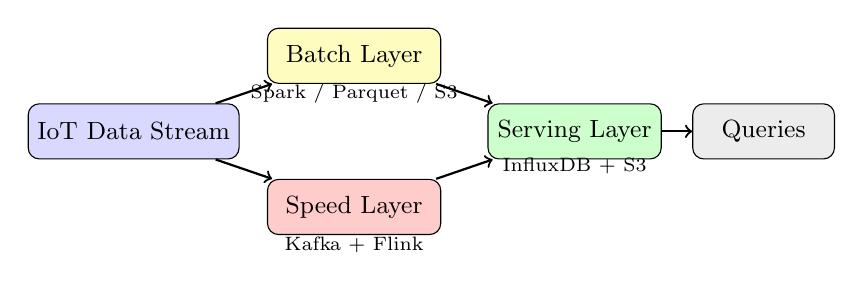
\begin{tikzpicture}[scale=0.8, every node/.style={font=\small}]
        % Input
        \node[draw, fill=blue!15, minimum width=1.8cm, minimum height=0.7cm, rounded corners] (input) at (0,0) {IoT Data Stream};

        % Batch layer
        \node[draw, fill=yellow!25, minimum width=2.2cm, minimum height=0.7cm, rounded corners] (batch) at (3.5,1.2) {Batch Layer};
        \node[font=\scriptsize] at (3.5,0.6) {Spark / Parquet / S3};

        % Speed layer
        \node[draw, fill=red!20, minimum width=2.2cm, minimum height=0.7cm, rounded corners] (speed) at (3.5,-1.2) {Speed Layer};
        \node[font=\scriptsize] at (3.5,-1.8) {Kafka + Flink};

        % Serving layer
        \node[draw, fill=green!20, minimum width=2.2cm, minimum height=0.7cm, rounded corners] (serve) at (7,0) {Serving Layer};
        \node[font=\scriptsize] at (7,-0.55) {InfluxDB + S3};

        % Output
        \node[draw, fill=gray!15, minimum width=1.8cm, minimum height=0.7cm, rounded corners] (out) at (10,0) {Queries};

        \draw[->, thick] (input) -- (batch);
        \draw[->, thick] (input) -- (speed);
        \draw[->, thick] (batch) -- (serve);
        \draw[->, thick] (speed) -- (serve);
        \draw[->, thick] (serve) -- (out);
    \end{tikzpicture}
    \end{center}

    \begin{columns}
        \column{0.5\textwidth}
        \textbf{Batch layer:} reprocesses all history. Accurate but slow (hours).

        \textbf{Speed layer:} real-time, recent data only. Fast but approximate.

        \column{0.5\textwidth}
        \textbf{Serving layer:} merges batch and speed views.

        \begin{alertblock}{Downside}
            Two codepaths = double maintenance. Kappa solves this.
        \end{alertblock}
    \end{columns}
\end{frame}

\begin{frame}{Kappa Architecture: Simplify with Streaming}
    \small
    \textbf{Kappa Architecture} (Jay Kreps, LinkedIn, 2014): one streaming pipeline.

    \vspace{0.05cm}
    \begin{columns}
        \column{0.5\textwidth}
        \textbf{Key idea:}
        \begin{itemize}\setlength{\itemsep}{0pt}
            \item \textbf{Remove} the batch layer
            \item \textbf{Replayable log} (Kafka) = source of truth
            \item Reprocessing = replay Kafka from offset~0
            \item Same code: real-time and historical queries
        \end{itemize}

        \vspace{0.05cm}
        \textbf{Why it works for IoT:}
        \begin{itemize}\setlength{\itemsep}{0pt}
            \item Kafka retains data for days/weeks
            \item Flink handles both streaming and batch
            \item Iceberg provides ACID on output lake
        \end{itemize}

        \column{0.5\textwidth}
        \textbf{Lambda vs Kappa:}
        \begin{center}
        \footnotesize
        \begin{tabular}{lcc}
            \toprule
            & \textbf{Lambda} & \textbf{Kappa} \\
            \midrule
            Codepaths & 2 & 1 \\
            Complexity & High & Lower \\
            Reprocessing & Full recompute & Kafka replay \\
            Latency & Low+High & Low \\
            Maturity & High & Growing \\
            \bottomrule
        \end{tabular}
        \normalsize
        \end{center}

        \begin{exampleblock}{2026 Trend}
            Confluent, AWS push Kappa via Kafka + Flink + Iceberg. Lambda dominant in legacy.
        \end{exampleblock}
    \end{columns}
\end{frame}

%==============================================================================
\section{Cloud IoT Platforms}
%==============================================================================

\begin{frame}{Cloud IoT Platforms in 2026: The Real Comparison}
    \vspace{0.05cm}
    \begin{center}
    \scriptsize
    \begin{tabular}{p{2.3cm}p{2.4cm}p{2.4cm}p{2.4cm}p{1.8cm}}
        \toprule
        & \textbf{AWS IoT Core} & \textbf{Azure IoT Hub} & \textbf{Google Cloud IoT} & \textbf{Self-hosted} \\
        \midrule
        \textbf{Protocol} & MQTT, HTTP, AMQP & MQTT, AMQP, HTTP & MQTT, HTTP & Any \\
        \textbf{Storage} & DynamoDB, S3, Timestream & Cosmos DB, Blob, ADX & BigQuery, Bigtable & Your choice \\
        \textbf{Edge} & Greengrass & IoT Edge & Edge TPU & K3s, EdgeX \\
        \textbf{Pricing} & Per message & Per message/day & Per message & CapEx \\
        \textbf{Lock-in} & High & High & High & None \\
        \textbf{Status 2026} & Dominant & Strong & GCP IoT Core \textbf{EOL 2023} & Growing \\
        \bottomrule
    \end{tabular}
    \normalsize
    \end{center}

    \begin{alertblock}{Google Cloud IoT Core was shut down August 2023}
        Customers migrated to AWS, Azure, or self-hosted EMQX/HiveMQ. Vendor lock-in risk is real.
    \end{alertblock}
\end{frame}

\begin{frame}{AWS IoT Data Stack (2026)}
    \small
    \textbf{AWS has the most complete IoT-to-storage pipeline:}

    \vspace{0.05cm}
    \begin{columns}
        \column{0.5\textwidth}
        \textbf{Ingestion:}
        \begin{itemize}\setlength{\itemsep}{0pt}
            \item AWS IoT Core: MQTT broker, rules engine
            \item Rules Engine: routes to 20+ AWS services
            \item Kinesis Data Streams: high-throughput ingest
        \end{itemize}

        \vspace{0.05cm}
        \textbf{Processing:}
        \begin{itemize}\setlength{\itemsep}{0pt}
            \item Kinesis Analytics (Flink): stream SQL
            \item AWS Lambda: serverless event processing
            \item AWS Glue: ETL for cold path
        \end{itemize}

        \column{0.5\textwidth}
        \textbf{Storage:}
        \begin{itemize}\setlength{\itemsep}{0pt}
            \item \textbf{Amazon Timestream}: managed TSDB
            \item \textbf{DynamoDB}: device state, last-known-value
            \item \textbf{S3 + Iceberg}: cold storage, data lake
            \item \textbf{OpenSearch}: log analytics
        \end{itemize}

        \vspace{0.05cm}
        \begin{alertblock}{Amazon Timestream (2026)}
            Auto-tiering: memory $\rightarrow$ S3. InfluxDB-compatible API. 1/10th the cost of DynamoDB for time-series.
        \end{alertblock}
    \end{columns}
\end{frame}

%==============================================================================
\section{Data Compression and Retention}
%==============================================================================

\begin{frame}{Data Compression for IoT}
    \small
    \textbf{Compression is not optional at IoT scale --- it's a design requirement.}

    \vspace{0.05cm}
    \begin{columns}
        \column{0.5\textwidth}
        \textbf{Time-series compression algorithms:}
        \begin{itemize}\setlength{\itemsep}{0pt}
            \item \textbf{Gorilla:} XOR delta-of-delta. 1.37~bytes/point. InfluxDB, Prometheus.
            \item \textbf{LZ4:} General fast. 400~MB/s decompression.
            \item \textbf{Snappy:} Moderate ratio, fast. Parquet, Cassandra.
            \item \textbf{Zstd:} Best ratio/speed. InfluxDB~3.x, Kafka.
        \end{itemize}

        \column{0.5\textwidth}
        \textbf{Practical compression ratios:}
        \begin{center}
        \footnotesize
        \begin{tabular}{lcc}
            \toprule
            \textbf{Format} & \textbf{Ratio} & \textbf{Use case} \\
            \midrule
            CSV & 1$\times$ & Baseline \\
            JSON & 0.8$\times$ & Worse than CSV \\
            Parquet & 5--20$\times$ & Cold storage \\
            Parquet+Zstd & 10--50$\times$ & Optimal cold \\
            Gorilla & 10$\times$ & Time-series DBs \\
            \bottomrule
        \end{tabular}
        \normalsize
        \end{center}

        \begin{exampleblock}{Bottom line}
            Storing raw JSON to S3 costs 10--50$\times$ more than Parquet+Zstd. At petabyte scale, that's millions of dollars per year.
        \end{exampleblock}
    \end{columns}
\end{frame}

\begin{frame}{Data Retention and Downsampling Policies}
    \small
    \textbf{You cannot keep raw sensor data forever. You need a retention strategy.}

    \vspace{0.05cm}
    \begin{columns}
        \column{0.5\textwidth}
        \textbf{Downsampling pyramid:}
        \begin{itemize}\setlength{\itemsep}{0pt}
            \item Raw (1~Hz): keep 7~days
            \item 1-min averages: keep 90~days
            \item 1-hr averages: keep 2~years
            \item 1-day averages: keep forever
        \end{itemize}

        \vspace{0.05cm}
        \textbf{InfluxDB continuous query:}\\
        \texttt{\scriptsize SELECT mean(temp) INTO "1h\_avg"."temp"}\\
        \texttt{\scriptsize FROM raw GROUP BY time(1h)}

        \vspace{0.05cm}
        \textbf{Cost impact:} Raw 1~Hz = 86,400 pts/sensor/day;
        1-hr avg = 24 pts/day $\Rightarrow$ \textbf{3,600$\times$ reduction}

        \column{0.5\textwidth}
        \textbf{Retention design considerations:}
        \begin{itemize}\setlength{\itemsep}{0pt}
            \item \textbf{Legal:} GDPR deletion, SCADA 10-yr retention
            \item \textbf{ML:} need 2+ years of raw data
            \item \textbf{Anomaly:} raw needed for event reconstruction
            \item \textbf{Billing:} smart meters need raw for disputes
        \end{itemize}

        \vspace{0.05cm}
        \begin{alertblock}{Design rule}
            Define retention policy before deployment. Retrofitting a billion-row table is painful.
        \end{alertblock}
    \end{columns}
\end{frame}

%==============================================================================
\section{Storage Selection Guide}
%==============================================================================

\begin{frame}{IoT Storage Selection Guide}
    \textbf{Same constraint-driven approach as protocol selection:}

    \vspace{0.05cm}
    \begin{center}
    \tiny
    \begin{tabular}{p{3.1cm}p{2.8cm}p{4.6cm}}
        \toprule
        \textbf{Dominant constraint} & \textbf{Technology} & \textbf{Reason} \\
        \midrule
        High-freq.~telemetry, real-time & \textbf{InfluxDB 3.x} & Purpose-built TSDB, Gorilla compression \\
        Time-series + relational JOINs & \textbf{TimescaleDB} & Full SQL, hypertables, aggregates \\
        Device state / last-known-value & \textbf{Redis} & Sub-ms reads, pub/sub built in \\
        Flexible schema, device metadata & \textbf{MongoDB} & Document model, Atlas Device Sync \\
        Cold storage, ML training & \textbf{S3 + Parquet + Iceberg} & 11-nines durability, 50$\times$ compression \\
        Edge, intermittent connectivity & \textbf{SQLite / QuestDB} & Embedded, zero-config, store-and-forward \\
        Multi-tenant hyperscale & \textbf{Cassandra / ScyllaDB} & Millions of writes/sec, linear scaling \\
        \bottomrule
    \end{tabular}
    \normalsize
    \end{center}

    \begin{alertblock}{No single winner}
        Production IoT systems use 3--4 storage technologies simultaneously, each optimized for its role.
    \end{alertblock}
\end{frame}

%==============================================================================
\section{State of the Art 2026}
%==============================================================================

\begin{frame}{State of the Art: IoT Data Storage in 2026}
    \small
    \begin{columns}
        \column{0.5\textwidth}
        \textbf{Established (production-ready):}
        \begin{itemize}\setlength{\itemsep}{0pt}
            \item \textbf{InfluxDB 3.x}: Parquet+S3 backend, SQL native
            \item \textbf{TimescaleDB}: continuous aggregates, data tiering
            \item \textbf{Apache Kafka}: immutable log, Kappa pattern
            \item \textbf{S3 + Parquet}: cold storage, DuckDB-queryable
            \item \textbf{AWS Timestream}: managed TSDB, S3 tiering
        \end{itemize}

        \column{0.5\textwidth}
        \textbf{Emerging (gaining traction):}
        \begin{itemize}\setlength{\itemsep}{0pt}
            \item \textbf{Apache Iceberg}: ACID lakehouses, replacing raw lakes
            \item \textbf{DuckDB}: in-process, queries S3 Parquet directly
            \item \textbf{InfluxDB IOx}: edge-deployable, same cloud API
            \item \textbf{RisingWave}: streaming SQL, materialized views
            \item \textbf{EdgeX Foundry}: open-source edge, pluggable storage
        \end{itemize}
    \end{columns}

    \vspace{0.05cm}
    \begin{alertblock}{Key trend: Storage-compute separation}
        Open formats (Parquet/Iceberg on S3). Query engines (DuckDB, Trino, Spark) attach on demand.
    \end{alertblock}
\end{frame}

%==============================================================================
\section{Summary}
%==============================================================================

\begin{frame}{Key Takeaways}
    \small
    \begin{columns}
        \column{0.5\textwidth}
        \textbf{Fundamentals:}
        \begin{itemize}\setlength{\itemsep}{0pt}
            \item 4~Vs: Volume, Velocity, Variety, Veracity
            \item Hot/warm/cold: design each hop separately
            \item TSDBs: optimized for sequential appends
            \item Gorilla: 10$\times$ space savings
        \end{itemize}

        \vspace{0.05cm}
        \textbf{Technologies:}
        \begin{itemize}\setlength{\itemsep}{0pt}
            \item InfluxDB~3.x: \#1 IoT TSDB, Parquet+S3
            \item TimescaleDB: SQL JOINs + time-series
            \item Redis: device state, sub-ms reads
            \item S3+Parquet+Iceberg: cold path, ML
        \end{itemize}

        \column{0.5\textwidth}
        \textbf{Architecture patterns:}
        \begin{itemize}\setlength{\itemsep}{0pt}
            \item Lambda: batch+speed, accurate, complex
            \item Kappa: streaming only, Kafka-based
            \item Edge-first: store locally, sync summaries
            \item Store-and-forward: survive outages
        \end{itemize}

        \vspace{0.05cm}
        \textbf{2026 trends:}
        \begin{itemize}\setlength{\itemsep}{0pt}
            \item Storage-compute separation (open formats)
            \item Apache Iceberg replacing raw data lakes
            \item Edge storage + selective cloud sync
        \end{itemize}
    \end{columns}

    \begin{alertblock}{The Meta-Lesson}
        Define retention, compression, and hot/warm/cold split \textbf{before} storing data.
    \end{alertblock}
\end{frame}

\begin{frame}{Questions?}
    \begin{center}
        \Huge Questions?

        \vspace{1cm}
        \normalsize
        \textbf{Eduardo Baena}\\
        \texttt{e.baena@northeastern.edu}\\[0.3cm]
        Module 7: Data Storage for IoT\\
        EECE5155 --- Spring 2026
    \end{center}
\end{frame}

\end{document}
